\chapter{Shrinkage Methods} \label{ch:shrinkageMethods}
Before we talked about methods that can be used to select the best subset of predictors. Shrinkage Methods regularizes or penalties the coefficient by shrinking the coefficients towards zero. Using this techniques that can reduce the variance. 

\section{Theory}

\subsection{Vector norm}

- Theory about the norm, zero, first, second, how we find it.
- Figure 6.7 in book. Connect this to ridge/lasso regression.

\subsection{Ridge regression}

The formula for Ridge regression can be seen in \ref{fo:RidgeRegression}. In blue we have the residual sum of square (RSS) term and in red we have the regularize or penalty term. The penalty term is small when $\beta_1, . ,\beta_p$ are close to zero and it has the effect of shrinking or penalizing the estimates of the coefficients $\beta_j$ towards zero. $\lambda$ also called a tuning parameter decides how much impact the two terms get. If $\lambda = 0$ then we will only get least squares estimates, but as $ \lambda \to \infty$ the penalty terms influence will increase and therefore the coefficients will approach zero. This means that the results will be different depending on the chosen $\lambda$ so for getting a good result picking the right $\lambda$ is important.

\noindent The penalty term only apply to the slope, not the intercept. $\lambda$ in in \ref{fo:RidgeRegression} control the degree of penalty.
\begin{align}\label{fo:RidgeRegression}
\color{blue} \sum_{i=1}^{n} ( y_i - \beta_0 - \sum_{j=1}^{p} \beta_j x_i,j )^2  \color{red} \lambda \sum_{j=1}^{p} \beta^2_j 
\end{align}
The reason to Ridge regression over least squares is found in the bias-variance
trade-off. This is because as our $\lambda$ gets bigger the complexity of the ridge regression fit decreases leading to less variance but more bias.

\subsection{The lasso regression}
The formula for least absolute shrinkage and selection operator, also called Lasso, can be seen in figure \ref{foTheLasso}. The blue part of the equation is the RSS (the ) and the red part is the penalty. The lasso regression has a advantage over Ridge regression because of the way the penalty term works. In Ridge it will include all $p_i$ predictors because the $\lambda \sum_{j=1}^{p} \beta^2_j$ only shrink all of the coefficients towards zero but not setting any of them to zero. In lasso we use as E \_ 1 norm of a coefficient vector $\beta$ is given by $ \lVert \beta_1 \rVert = \sum | \beta_j |$ which makes some of the coefficient estimates to be exactly zero when the tuning parameter $\lambda$ is large enough.
\begin{align}\label{fo:TheLasso}
\color{blue} \sum_{i=1}^{n} ( y_i - \beta_0 - \sum_{j=1}^{p} \beta_j x_i,j )^2  \color{red} \lambda \sum_{j=1}^{p} |\beta_j|
\end{align}
Because the lasso regression removes some of the coefficients, lasso models are generally easier to understand than Ridge regression ones because they are  more sparse with a reduced complexity. Lasso models involve only a subset of the variables. As before selecting a good $\lambda$ is again important here.

\subsection{Comparing ridge and lasso regression}

- Show here which is better when. MSE? RSS? What makes one superior to the other?


\begin{figure}[H]
	\centering
	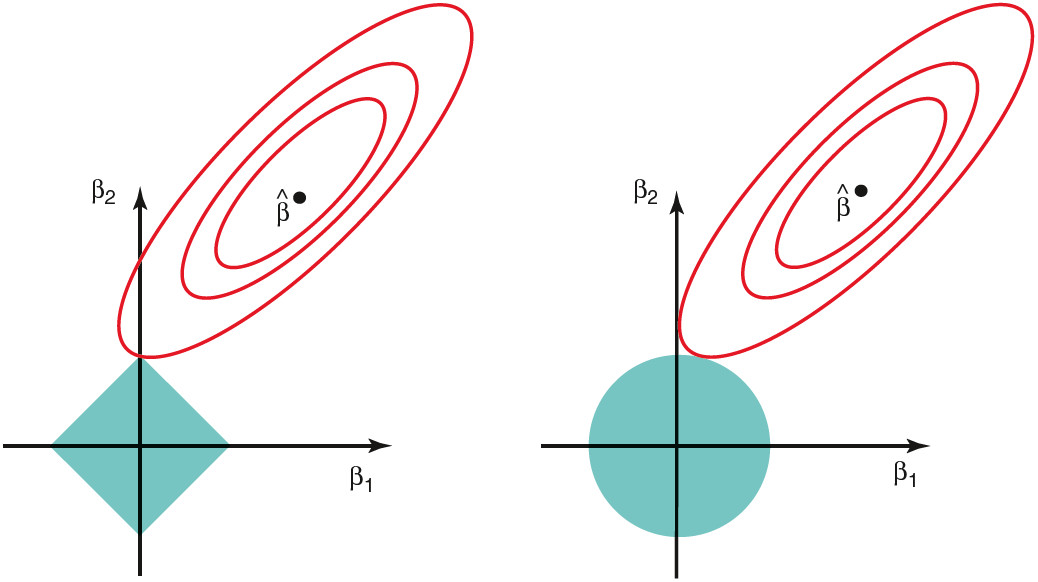
\includegraphics[width=0.3\textwidth]{shrinkageMethods/fig/normsL1_L2.jpg}
	\caption{The red eclipse shows the concurs of ridge (left) and lasso (right) regression. The blue areas are constraint regions for the first and second norm. Notice that lasso intersects the constraint region at an axis, whereas ridge does not.}
	\label{fig:normfirstsecond}
\end{figure}

\section{Results}

- Labs here.
- Show MSE. Compare. Use bootstrap. Explain why lasso/ridge is better and when.